\StartPlate{V16}{Central normalization of a descent fibre}{A power map can be bijective in one fibre and collapse an entire family in another.}
\begin{center}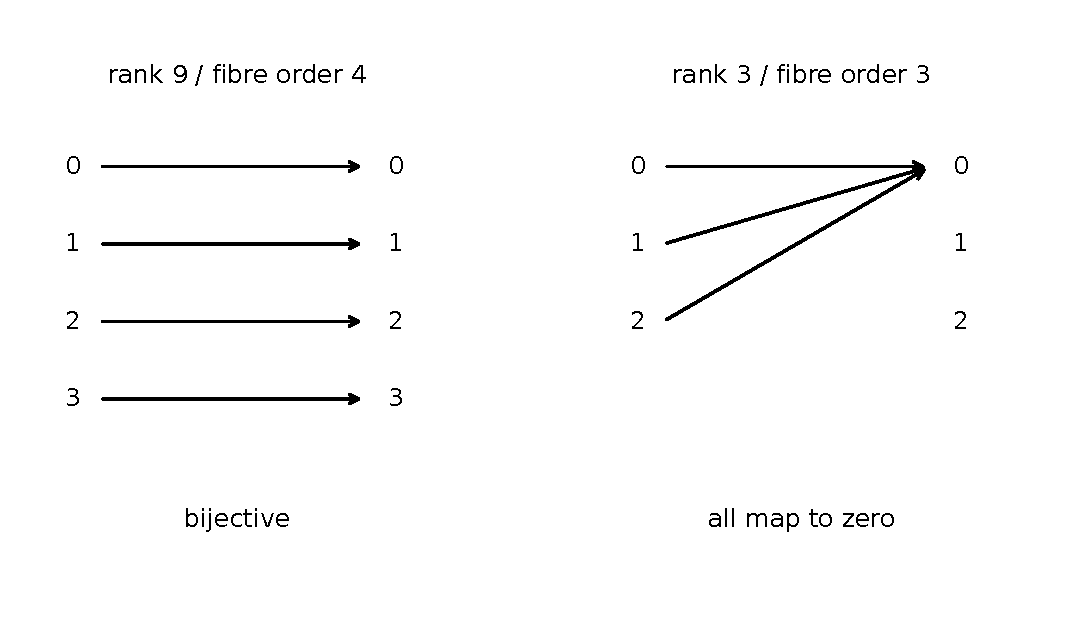
\includegraphics[width=\linewidth]{figures/V16.pdf}\end{center}
A descent fibre that is a torsor for a cyclic character group $X$ of order $m$ is normalized by the central-character power map $\alpha\mapsto\alpha^n$. Additive exponents identify it with $x\mapsto nx\pmod m$.

On the left, $n=9$ and $m=4$. The map is the identity modulo four, so every attainable central-character ratio selects one twist. On the right, $n=3$ and $m=3$. Every exponent maps to zero, so the fixed-center condition leaves all three twists available.
\[
\gcd(n,m)=1\quad\Longrightarrow\quad
\text{unique member for each attainable central ratio.}
\]
The two examples correspond to different source branches. The rank-nine positive-characteristic descent and the rank-three continuation113 fixed-center ambiguity are not one candidate under two names. Uniqueness in the coprime fibre does not prove a native character occurs in that candidate. Ambiguity in the cubic fibre does not disappear because a scalar obstruction has been removed.
\vfill\PlateSource{Exact finite character-group model}{Part II, Sections 17.3 and 18.4; Part III, Section 25.3}{46}
